% Chuong 5  --  phu trach: Dung (xem report/PHANCONG.md)
% Moi muc la mot file s*.tex trong thu muc nay, de nhieu nguoi sua song song khong dung nhau.
% nguon: rtl/cnn1d/comm/, rtl/cnn1d/top/layer_cmd_controller.v, python/link/, host/, docs/baseline_v1.md
\chapter{Giao thức giao tiếp Host--Accelerator}\label{ch:uart}

Chương này mô tả kênh giao tiếp nối tiếp và giao thức điều khiển giữa máy chủ (host) và bộ tăng tốc trên FPGA.
Mục~\ref{sec:uartvl} trình bày tầng vật lý UART, bộ chia tốc độ baud và cơ chế lấy mẫu bit.
Mục~\ref{sec:khungoi} mô tả cấu trúc khung gói hai chiều, kiểm lỗi CRC-16 và giới hạn tải tối đa.
Mục~\ref{sec:bolenh} giải thích lý do thiết kế bộ lệnh ở mức layer cùng các cờ mở rộng cho hai lớp kết nối đầy đủ và chế độ trọng số thường trú.
Mục~\ref{sec:fsmuart} phân tích máy trạng thái dừng--chờ, cách xử lý lỗi và quy tắc quản lý các bank nhớ ping-pong.
Mục~\ref{sec:trinhtu} tổng hợp trình tự lệnh phân loại một nhịp tim kèm chi phí đường truyền; Mục~\ref{sec:phiahost} trình bày ngăn xếp phần mềm phía host, mô hình giả lập mức byte và các công cụ kiểm chứng trên board.
Mã nguồn tương ứng nằm tại \texttt{rtl/cnn1d/comm/}, \texttt{rtl/cnn1d/top/layer\_cmd\_controller.v}, \texttt{python/link/} và \texttt{host/}.

% Muc 5.1  --  phu trach: Dung (xem report/PHANCONG.md)
% nguon: rtl/cnn1d/de10_lite_top.v, rtl/cnn1d/top/ecg_accel_top.v, rtl/cnn1d/comm/uart/uart_rx.v, uart_tx.v
\section{Tầng vật lý UART}\label{sec:uartvl}
Host kết nối với board DE10-Lite qua bộ thu phát không đồng bộ vạn năng (Universal Asynchronous Receiver/Transmitter, UART) mức logic $3{,}3$~V thông qua cầu chuyển đổi USB--UART CH340.
Giao diện trên FPGA (\texttt{de10\_lite\_top}) gồm chân thu \texttt{uart\_rx} (\texttt{PIN\_AB5}), chân phát \texttt{uart\_tx} (\texttt{PIN\_AB6}) và đất chung, truyền theo định dạng \emph{8N1} ($1$~bit start mức~$0$, $8$~bit dữ liệu từ bit thấp trước, $1$~bit stop mức~$1$) không dùng điều khiển luồng phần cứng.
Mạch vận hành với xung nhịp hệ thống \texttt{CLK\_FREQ} $=50$~MHz và tốc độ truyền \texttt{BAUD\_RATE} $=1\,500\,000$~baud (hỗ trợ cấu hình ở $921\,600$~baud và $1\,500\,000$~baud), chia chu kỳ bit theo $\texttt{DIV}=\lfloor\texttt{CLK\_FREQ}/\texttt{BAUD\_RATE}\rfloor$ với điều kiện thiết kế $\texttt{CLK\_FREQ}/\texttt{BAUD\_RATE}\ge8$.

Module thu \texttt{uart\_receiver} (\texttt{comm/\allowbreak uart/\allowbreak uart\_rx.v}) đồng bộ tín hiệu \texttt{rx\_in} qua hai tầng thanh ghi liên tiếp (\texttt{rx\_meta}, \texttt{rx\_sync}), sau đó giải mã byte bằng máy trạng thái hữu hạn (Finite State Machine, FSM) năm trạng thái: \texttt{IDLE}, \texttt{START}, \texttt{DATA}, \texttt{STOP} và \texttt{RECOVER}.
Khi gặp cạnh xuống ở \texttt{IDLE}, mạch sang \texttt{START} và đếm nửa chu kỳ bit ($\texttt{DIV}/2-1$) để kiểm tra tại tâm bit start: nếu đường dây về mức~$1$ sớm thì loại bỏ start giả và quay lại \texttt{IDLE}; nếu giữ mức~$0$ thì chuyển sang \texttt{DATA} lấy mẫu $8$~bit dữ liệu cách đều mỗi $\texttt{DIV}$ chu kỳ.
Tại \texttt{STOP}, mạch lấy mẫu tâm bit stop: nếu bằng~$1$ thì xuất \texttt{data\_out} kèm xung \texttt{rx\_ready}; nếu bằng~$0$ thì phát xung \texttt{frame\_error} và đợi ở \texttt{RECOVER} cho tới khi đường dây trở về mức nghỉ~$1$.
Ở chiều ngược lại, \texttt{uart\_transmitter} (\texttt{comm/\allowbreak uart/\allowbreak uart\_tx.v}) nhận byte mới khi cờ \texttt{tx\_ready} bật, dịch nối tiếp bit start, $8$~bit dữ liệu và giữ đủ trọn độ rộng bit stop trước khi hoàn tất khung.

% Muc 5.2  --  phu trach: Dung (xem report/PHANCONG.md)
% nguon: rtl/cnn1d/comm/crc/crc16_ccitt_next.v, comm/protocol/packet_rx.v, packet_tx.v
\section{Khung gói và CRC-16}\label{sec:khungoi}
Mọi gói tin trao đổi trên cả hai chiều giữa host và bộ tăng tốc đều dùng chung định dạng khung trên Hình~\ref{fig:khungoi}, với các trường nhiều byte xếp theo thứ tự byte thấp trước (little-endian).

\begin{figure}[htbp]\centering
  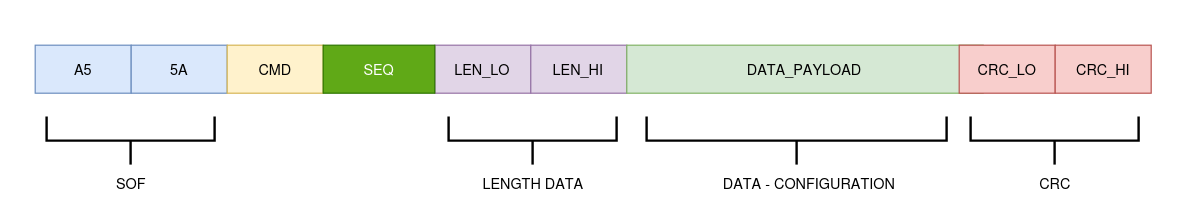
\includegraphics[width=0.96\textwidth]{ch05_giao_thuc_uart/frame.png}
  \caption{Cấu trúc khung gói UART.}\label{fig:khungoi}
\end{figure}

Khung gói gồm $8$~byte bao gói cố định và phần tải dữ liệu:
\begin{itemize}
  \item \textbf{\texttt{SOF} (\texttt{0xA5}, \texttt{0x5A}):} $2$~byte đồng bộ đầu khung; phần thân gói được đếm theo độ dài \texttt{LEN} nên các byte trùng giá trị \texttt{SOF} trong vùng tải vẫn truyền bình thường.
  \item \textbf{\texttt{CMD} và \texttt{SEQ} ($1$~byte mỗi trường):} \texttt{CMD} mang mã lệnh ở chiều xuống (\texttt{0x08}--\texttt{0x15}) hoặc loại trả lời ở chiều lên (\texttt{0x80} \texttt{ACK}, \texttt{0x81} \texttt{NACK}, \texttt{0x82} \texttt{RESULT}); \texttt{SEQ} là số thứ tự gói do host cấp và được FPGA sao chép lại vào khung trả lời.
  \item \textbf{\texttt{LENGTH DATA} (\texttt{LEN\_LO}, \texttt{LEN\_HI}):} độ dài tải kiểu \texttt{u16} ($0\le\texttt{LEN}\le\texttt{MAX\_PAYLOAD}$).
  \item \textbf{\texttt{DATA\_PAYLOAD} (\texttt{LEN}~byte):} chứa địa chỉ, tham số cấu hình hoặc dữ liệu truyền nhận; bỏ qua khi $\texttt{LEN}=0$.
  \item \textbf{\texttt{CRC} (\texttt{CRC\_LO}, \texttt{CRC\_HI}):} mã kiểm tra dư thừa vòng (Cyclic Redundancy Check, CRC) $16$~bit tính từ byte \texttt{CMD} đến hết \texttt{DATA\_PAYLOAD}.
\end{itemize}

Cả chiều thu và chiều phát đều dùng chuẩn CRC-16/CCITT-FALSE (đa thức \texttt{0x1021}, giá trị khởi tạo \texttt{0xFFFF}) thông qua mạch tổ hợp \texttt{crc16\_ccitt\_next} (\texttt{comm/\allowbreak crc/\allowbreak crc16\_ccitt\_next.v}) cập nhật một byte mỗi chu kỳ xung nhịp.
Trong \texttt{packet\_rx} (\texttt{comm/\allowbreak protocol/\allowbreak packet\_rx.v}), các byte tải được ghi vào thanh ghi đệm tạm và chỉ phát xung \texttt{packet\_valid} sau khi kiểm khớp hai byte CRC cuối gói; nếu vượt \texttt{MAX\_PAYLOAD} hoặc sai CRC, mạch phát xung \texttt{packet\_error} để bộ điều khiển trả tín hiệu từ chối (Negative Acknowledge, NACK) mã~$1$ mà không ghi vào bộ nhớ truy cập ngẫu nhiên tĩnh (Static Random-Access Memory, SRAM).
Khi đang nhận dở một khung mà không có byte mới trong khoảng \texttt{RX\_TIMEOUT\_CLKS} ($\texttt{CLK\_FREQ}/10$) hoặc có xung \texttt{frame\_error}, \texttt{packet\_rx} tự đưa trạng thái về chờ \texttt{0xA5}.

Tham số \texttt{MAX\_PAYLOAD} của thiết kế là $128$~byte (trả trọn $64$~giá trị $16$~bit của bộ nhớ trung bình toàn cục --- Global Average Pooling, GAP --- trong một khung).
Đối với các lệnh ghi mảng có $2$~byte địa chỉ ở đầu tải, mỗi gói mang tối đa $126$~byte dữ liệu và các mảng lớn hơn được host tự động tách thành nhiều khung nối tiếp.

% Muc 5.3  --  phu trach: xem report/PHANCONG.md
\section{Bộ lệnh}\label{sec:bolenh}
\begin{goiy}
  \begin{itemize}
    \item Nạp dữ liệu: \texttt{WRITE\_X} 0x08, \texttt{WRITE\_W} 0x09, \texttt{WRITE\_BIAS} 0x0A, \texttt{WRITE\_SHIFT} 0x0B, \texttt{SWAP} 0x0C.
    \item Chạy layer: \texttt{CONFIG} 0x0D (\texttt{out\_len, cout, k\_len, window\_step, pool, gap, pad\_next}, cờ, \texttt{w\_base, b\_base}), \texttt{RUN} 0x0E.
    \item Đọc: \texttt{READ\_GAP} 0x0F, \texttt{READ\_FMAP} 0x10, \texttt{INFO} 0x15 (phần cứng tự khai báo cấu hình).
    \item Cờ CONFIG: \texttt{out\_int32}, \texttt{argmax}, \texttt{row\_combine}, \texttt{gap\_in}; các ràng buộc hợp lệ (NACK mã 2).
    \item Bảng đầy đủ lệnh/tham số/phản hồi (Bảng~\ref{tab:lenh}; chi tiết ở Phụ lục~\ref{pl:bolenh}).
  \end{itemize}
\end{goiy}
\bangcho{mã lệnh · tham số · phản hồi · tác dụng}{Bộ lệnh điều khiển accelerator.}{tab:lenh}

% Muc 5.4  --  phu trach: xem report/PHANCONG.md
\section{Máy trạng thái và xử lý lỗi}\label{sec:fsmuart}
\begin{goiy}
  \begin{itemize}
    \item Stop-and-wait: mỗi lệnh một phản hồi 0x80 ACK, 0x81 NACK (mã lỗi 1 khung/CRC, 2 tham số sai, 3 sai trạng thái), 0x82 RESULT.
    \item Host không tự gửi lại sau timeout/NACK (lệnh có thể không idempotent); cách phục hồi.
    \item Quản lý quyền sở hữu bank ghi/đọc (ping-pong) và \texttt{SWAP}.
  \end{itemize}
\end{goiy}

% Muc 5.5  --  phu trach: Dung (xem report/PHANCONG.md)
% nguon: host/board_classifier.py, host/ecg_layer_host_pc.py
\section{Trình tự thực thi một nhịp}\label{sec:trinhtu}
Để phân loại một nhịp tim, host điều phối bộ tăng tốc theo ba giai đoạn như Hình~\ref{fig:trinhtu}: nạp tín hiệu đầu vào, lặp thực thi từng layer, và đọc kết quả.

\begin{figure}[htbp]\centering
  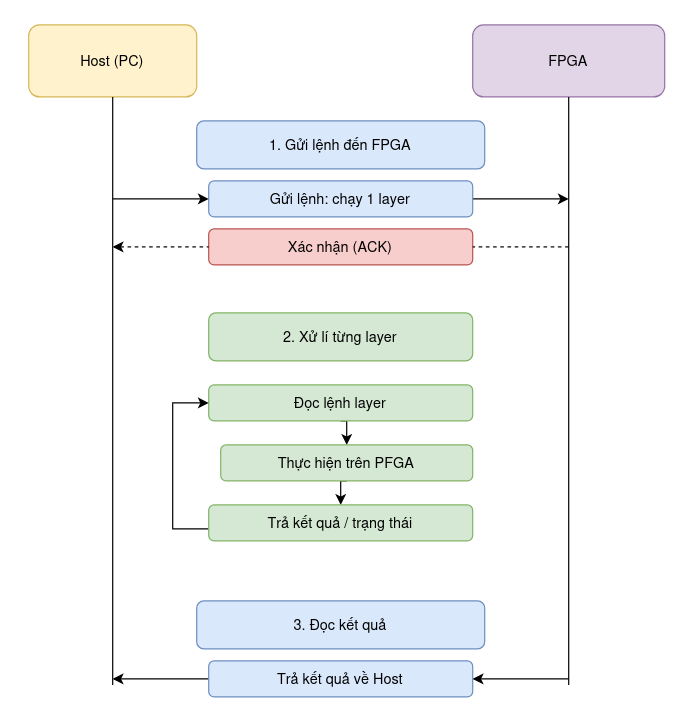
\includegraphics[width=0.7\textwidth]{ch05_giao_thuc_uart/trinh_tu.png}
  \caption{Trình tự lệnh giữa host và FPGA cho một nhịp.}\label{fig:trinhtu}
\end{figure}

\begin{enumerate}
  \item \textbf{Nạp tín hiệu đầu vào.} Host ghi cửa sổ tín hiệu của nhịp vào bộ nhớ ifmap bằng \texttt{WRITE\_X}, sau đó gọi \texttt{SWAP} để dữ liệu này trở thành bank đọc. Mỗi lệnh được FPGA xác nhận bằng \texttt{ACK}.
  \item \textbf{Lặp thực thi từng layer.} Với mỗi layer trong sáu layer của mạng (\texttt{conv0}, \texttt{conv1}, \texttt{conv2}, \texttt{conv3}, \texttt{FC1}, \texttt{FC2}), host gửi \texttt{WRITE\_SHIFT}, \texttt{CONFIG} và \texttt{RUN}. FPGA tính toán trên dữ liệu nằm sẵn trong bộ nhớ trên chip rồi trả về \texttt{RESULT} chứa trạng thái; đầu ra của layer này là đầu vào của layer sau nên không phải đọc về host. Riêng \texttt{FC1} cần thêm đặc trưng RR do host ghi bằng \texttt{WRITE\_X}, và \texttt{FC2} bật cờ \texttt{out\_int32} cùng \texttt{argmax}.
  \item \textbf{Đọc kết quả.} Host gửi \texttt{READ\_FMAP} để nhận logit và nhãn dự đoán của lớp đầu ra.
\end{enumerate}

Tham số của mô hình (trọng số, bias) có thể được cấp theo hai cách do phần mềm host lựa chọn:
\begin{itemize}
  \item \textbf{Gửi lại theo từng layer:} trước mỗi layer, host ghi trọng số và bias của layer đó vào bộ nhớ.
  \item \textbf{Nạp một lần (\texttt{--resident}):} host ghi toàn bộ trọng số và bias của mạng vào hai bank trọng số và bộ nhớ bias ngay từ đầu. Mỗi layer sau đó dùng \texttt{w\_base} và \texttt{b\_base} trong \texttt{CONFIG} để trỏ đến vùng tham số của mình, và host chỉ dùng \texttt{SWAP} đổi bank trọng số đọc giữa các nhóm layer. Cách này loại bỏ việc gửi lại tham số ở mỗi nhịp.
\end{itemize}

% Muc 5.6  --  phu trach: Dung (xem report/PHANCONG.md)
% nguon: python/link/serial_link.py, proto_layer.py, layer_host.py, layersim/, host/, scripts/board_*.py
\section{Phía host}\label{sec:phiahost}
Phần mềm phía host được tổ chức thành hai khối dùng chung một giao diện điều khiển cho cả kết nối phần cứng lẫn mô phỏng:
\sloppy
\begin{itemize}
  \item \textbf{Giao vận và điều phối mô hình (\texttt{python/\allowbreak link/}, \texttt{host/}):} \texttt{SerialTransport} đảm nhận truyền nhận byte qua cổng nối tiếp 8N1 (kèm \texttt{RawLog} lưu nhật ký byte thô); \texttt{LayerHost} đóng khung gói, tính/kiểm CRC-16, kiểm khớp \texttt{SEQ}, truy vấn \texttt{INFO} và tự động cắt gói theo \texttt{MAX\_PAYLOAD}. Phía trên, \texttt{ecg\_layer\_host\_pc.py} chạy kiểm tra từng layer và đọc lại đầu ra để đối chiếu với vector chuẩn, còn \texttt{board\_classifier.py} (\texttt{BoardClassifier}) điều phối chạy trọn sáu layer và chỉ đọc $17$~byte kết quả cuối cho mỗi nhịp.
  \item \textbf{Mô hình giả lập và công cụ vận hành (\texttt{python/\allowbreak link/\allowbreak layersim}, \texttt{scripts/}):} gói \texttt{layersim} (\texttt{LayerFpgaSim}, \texttt{LayerLink}) mô phỏng hoạt động thu phát khung, giải mã lệnh và tính toán số nguyên của FPGA ở mức byte. Các công cụ dòng lệnh dùng chung giao diện gồm \texttt{layer\_board\_test.py} (truy vấn \texttt{INFO} và kiểm tra khói), \texttt{board\_monitor.py} (chạy tiền xử lý trên host, gọi FPGA ở luồng nền để hiển thị trực tiếp và kiểm tra tự động \texttt{--check all}), \texttt{board\_compare.py} (hiển thị đối chiếu trực tiếp nhãn PhysioNet, mô hình số thực và FPGA), và \texttt{board\_eval.py} (phân loại và xuất kết quả đánh giá cho cả bản ghi MIT-BIH).
\end{itemize}
\fussy

